\documentclass{article}

\usepackage[letterpaper,portrait,top=0.4in, left=0.6in, right=0.6in, bottom=1in]{geometry}

\usepackage{amsmath, amsfonts, amsthm, amssymb}
\usepackage{graphicx, float}
\usepackage{mathtools}
\usepackage{titlesec}
\usepackage{interval}
\usepackage{hyperref}
\usepackage{siunitx}
\usepackage{titling}
\usepackage{vwcol}
\usepackage{setspace}
\usepackage{empheq}
\usepackage{cancel}
\usepackage{esdiff}
\usepackage{multicol}
\usepackage{mdframed}
\usepackage{esdiff}
\usepackage{tikzsymbols}
\usepackage{multicol}
\usepackage{tikz}
\usepackage{varwidth}

\intervalconfig {
	soft open fences
}

\newcommand{\alignedintertext}[1]{%
  \noalign{%
    \vskip\belowdisplayshortskip
    \vtop{\hsize=\linewidth#1\par
    \expandafter}%
    \expandafter\prevdepth\the\prevdepth
  }%
}

\renewcommand\qedsymbol{\Smiley[1.3]}
\newcommand*{\paren}[1]{\ensuremath\left(#1\right)}
\newcommand*{\problem}[1]{\section*{Problem #1}}
\newcommand*{\limit}[2][x]{\ensuremath{\displaystyle\lim_{#1\to#2}}}
\newcommand*{\Limit}[3][x]{\ensuremath{\displaystyle\lim_{#1\to#2}\left[#3\right]}}
\newcommand*{\deriv}[1][x]{\ensuremath{\dfrac{\mathrm{d}}{\mathrm{d}#1}}}
\newcommand*{\Deriv}[2][x]{\ensuremath{\dfrac{\mathrm{d}}{\mathrm{d}#1}\left[#2\right]}}

\DeclareMathOperator{\DNE}{DNE}

%opening
\title{Problem Set \#55}
\author{Jayden Li}
\date{March 21, 2024}

\allowdisplaybreaks

\begin{document}
\setstretch{1.25}
\fontsize{12pt}{12pt}\selectfont
\setlength{\abovedisplayskip}{0pt}
\maketitle

\problem{2}
\begin{itemize}
	\item[(a)]
	Yes.
	\begin{proof}
		Let $f(x)=\dfrac{|x|}{x}$ and $g(x)=-\dfrac{|x|}{x}$. Then $f(x)+g(x)=\dfrac{|x|}{x}+\paren{-\dfrac{|x|}{x}}=0$ for all $x\neq0$.
		\begin{gather*}
			\limit{0^+}f(x)=1,\limit{0^-}f(x)=-1\implies\limit{0}f(x)\DNE \\
			\limit{0^+}g(x)=-1,\limit{0^+}g(x)=1\implies\limit{0}g(x)\DNE \\
			\Limit{0}{f(x)+g(x)}=\limit{0}0=0
		\end{gather*}
	\end{proof}

	\item[(b)]
	Yes.
	\begin{proof}
		Let $L=\limit{a^+}f(x)=\limit{a^-}f(x)=\limit{a}f(x)$. Because $\Limit{a}{f(x)+g(x)}$ exists:
		\begin{gather*}
			 \Limit{a^+}{f(x)+g(x)}=\Limit{a^-}{f(x)+g(x)}=\Limit{a}{f(x)+g(x)} \\
			\limit{a^+}f(x)+\limit{a^+}g(x)=\limit{a^-}f(x)+\limit{a^-}g(x)=\limit{a}f(x)+\limit{a}g(x) \\
			L+\limit{a^+}g(x)=L+\limit{a^-}g(x)=L+\limit{a}g(x) \\
			\limit{a^+}g(x)=\limit{a^-}g(x)=\limit{a}g(x)
		\end{gather*}
		Therefore $\limit{a}g(x)$ must exist.
	\end{proof}

	\item[(c)]
	No.
	\begin{proof}
		Let $L=\limit{a^+}f(x)=\limit{a^-}f(x)=\limit{a}f(x)$. Because $\limit{a}g(x)\DNE$:
		\begin{align*}
			\limit{a^+}g(x)&\neq\limit{a^-}g(x) \\
			L+\limit{a^+}g(x)&\neq L+\limit{a^-}g(x) \\
			\limit{a^+}f(x)+\limit{a^+}g(x)&\neq\limit{a^-}f(x)+\limit{a^-}g(x) \\
			\Limit{a^+}{f(x)+g(x)}&\neq\Limit{a^-}{f(x)+g(x)} \\
		\end{align*}
		Therefore $\Limit{a}{f(x)+g(x)}\DNE$.
	\end{proof}
\end{itemize}

\problem{3}
\begin{multicols}{2}
\begin{itemize}
	\item[(b)]
	$\begin{aligned}[t]
		&\limit{0}\frac{\tan^2x+2x}{x+x^2} \\
		={}&\limit{0}\frac{\sin^2x+2x\cos^2x}{x^2\paren{\frac{1}{x}+1}\cos^2x} \\
		={}&\Limit{0}{\frac{\sin^2x}{x^2\paren{\frac{1}{x}+1}\cos^2x}+\frac{2x\cancel{\cos^2x}}{x^2\paren{\frac{1}{x}+1}\cancel{\cos^2x}}} \\
		={}&\Limit{0}{\frac{\sin^2x}{x^2}\cdot\frac{1}{\paren{\frac{1}{x}+1}\cos^2x}}+\limit{0}\frac{2}{1+x} \\
		={}&\paren{\limit{0}\frac{\sin x}{x}}^2\limit{0}\frac{1}{\frac{(1+x)\cos^2x}{x}}\limit{0}\frac{1}{\cos^2x}+2 \\
		={}&1^2\cdot\Limit{0}{\frac{x}{(1+x)\cos^2x}}\cdot\frac{1}{1^2}+2 \\
		={}&\boxed{2}
	\end{aligned}$

	\item[(d)]
	$\begin{aligned}[t]
		&\limit[h]{0}\frac{\sin(x+h)-\sin x}{h} \\
		={}&\limit[h]{0}\frac{\sin x\cos h+\cos x\sin h-\sin x}{h} \\
		={}&\limit[h]{0}\frac{\sin(x)(\cos h-1)+\cos x\sin h}{h} \\
		={}&\limit[h]{0}\frac{\sin(x)(\cos h-1)}{h}+\limit[h]{0}\frac{\cos x\sin h}{h} \\
		={}&\limit[h]{0}\frac{\cos h - 1}{h}\limit[h]{0}\sin x+\limit[h]{0}\frac{\sin h}{h}\limit[h]{0}\cos x \\
		={}&0\cdot\sin x+1\cdot\cos x \\
		={}&\boxed{\cos x}
	\end{aligned}$
\end{itemize}
\end{multicols}

\problem{4}
\begin{multicols}{2}
\begin{itemize}
	\item[(b)]
	$\begin{aligned}[t]
		&\limit{\infty}x\sin\paren{\frac{1}{x}} \\
		={}&\Limit{\infty}{\frac{x\sin\paren{\frac{1}{x}}}{\frac{1}{x}}\cdot\frac{1}{x}} \\
		={}&\limit{\infty}\frac{\sin\paren{\frac{1}{x}}}{\frac{1}{x}}\Limit{\infty}{x\cdot\frac{1}{x}} \\
		\alignedintertext{Let $y=\frac{1}{x}$. As $x\to\infty$, $y\to0$.}
		={}&\limit[y]{0}\frac{\sin(y)}{y}\limit{\infty}1 \\
		={}&\boxed{1}
	\end{aligned}$

	\item[(d)]
	$\begin{aligned}[t]
		&\limit{\infty}\frac{x\sin x}{x^2+5} \\
		={}&\limit{\infty}\frac{\cancel{x^2}\paren{\frac{\sin x}{x^2}}}{\cancel{x^2}\paren{1+\frac{5}{x^2}}} \\
		={}&\frac{\limit{\infty}\frac{\sin x}{x}\limit{\infty}\frac{1}{x}}{\limit{\infty}1+\limit{\infty}\frac{5}{x^2}} \\
		={}&\frac{0\cdot0}{1+0} \\
		={}&\boxed{0}
	\end{aligned}$
\end{itemize}
\end{multicols}

\pagebreak
\problem{5}
\begin{multicols}{2}
\begin{itemize}
	\item[(b)]
	$\begin{aligned}[t]
		&\limit{\infty}x(1+\sin^2x) \\
		={}&\limit{\infty}x+\limit{\infty}x\sin^2x \\
		\alignedintertext{$\limit{\infty}x\sin^2x$ oscillates on the interval $\interval[open right]{0}{\infty}$.}
		={}&\boxed{\infty}
	\end{aligned}$

	\item[(d)]
	$\begin{aligned}[t]
		&\limit{\infty}x^2\sin\paren{\frac{1}{x}} \\
		={}&\Limit{\infty}{\frac{x^2\sin\paren{\frac{1}{x}}}{\frac{1}{x}}\cdot\frac{1}{x}} \\
		={}&\limit{\infty}\frac{\sin\paren{\frac{1}{x}}}{\frac{1}{x}}\Limit{\infty}{x^2\cdot\frac{1}{x}} \\
		\alignedintertext{Let $y=\frac{1}{x}$. As $x\to\infty$, $y\to0$.}
		={}&\limit[y]{0}\frac{\sin(y)}{y}\limit{\infty}x \\
		={}&\boxed{\infty}
	\end{aligned}$

	\item[(e)]
	$\begin{aligned}[t]
		&\Limit{\infty}{\sqrt{x^2+2x}-x} \\
		={}&\limit{\infty}\frac{\paren{\sqrt{x^2+2x}-x}\paren{\sqrt{x^2+2x}+x}}{\sqrt{x^2+2x}+x} \\
		={}&\limit{\infty}\frac{x^2+2x-x^2}{\sqrt{x^2}\sqrt{1+\frac{2}{x}}+x} \\
		={}&\limit{\infty}\frac{2x}{|x|\sqrt{1+\frac{2}{x}}+x} \\
		\alignedintertext{Because $x\to\infty$, $x$ is positive.}
		={}&\limit{\infty}\frac{2\cancel{x}}{\cancel{x}\sqrt{1+\frac{2}{x}}+\cancelto{1}{x}} \\
		={}&\limit{\infty}\frac{2}{\sqrt{1+0}+1} \\
		={}&\boxed{1}
	\end{aligned}$

	\item[(f)]
	$\begin{aligned}[t]
		&\Limit{\infty}{x(\sqrt{x+2}-\sqrt{x})} \\
		={}&\limit{\infty}\frac{x(\sqrt{x+2}-\sqrt{x})(\sqrt{x+2}+\sqrt{x})}{\sqrt{x+2}+\sqrt{x}} \\
		={}&\limit{\infty}\frac{x(x+2-x)}{\sqrt{x+2}+\sqrt{x}} \\
		={}&\limit{\infty}\frac{2x}{\sqrt{x+2}+\sqrt{x}} \\
		={}&\limit{\infty}\frac{2x}{\sqrt{x^2\paren{\frac{1}{x}+\frac{2}{x^2}}}+\sqrt{x^2\paren{\frac{1}{x}}}} \\
		={}&\limit{\infty}\frac{2x}{|x|\paren{\sqrt{\frac{1}{x}+\frac{2}{x^2}}+\sqrt{\frac{1}{x}}}} \\
		\alignedintertext{$x$ is positive. As $x\to\infty$, $\frac{1}{x}$ and $\frac{2}{x^2}$ are positive and approach $0$ but do not equal $0$.}
		={}&\limit{\infty}\frac{2}{\sqrt{\frac{1}{x}+\frac{2}{x^2}}+\sqrt{\frac{1}{x}}} \\
		\alignedintertext{The denominator is positive and approaches $0$. A positive real number divided by a positive number approaching $0$ is $\infty$.}
		={}&\boxed{\infty}
	\end{aligned}$

	\item[(g)]
	$\begin{aligned}[t]
		&\limit{\infty}\frac{\sqrt{|x|}}{x} \\
		\alignedintertext{$x$ is positive.}
		={}&\limit{\infty}\frac{\sqrt{x}}{|x|} \\
		={}&\limit{\infty}\frac{\sqrt{x}}{\sqrt{x^2}} \\
		={}&\limit{\infty}\sqrt{\frac{1}{x}} \\
		={}&\boxed{0}
	\end{aligned}$
\end{itemize}
\end{multicols}

\pagebreak
\problem{6}
\begin{itemize}
	\item[(a)]
	\phantom{}

	\begin{minipage}[t]{0.5\linewidth}
		\begin{align*}
			\angle QOP&=\frac{2\pi}{n} \\
			\angle QPO=\angle PQO&=\frac{1}{2}\paren{\ang{180}-\frac{2\pi}{n}} \\
			&=\frac{\pi}{2}-\frac{\pi}{n} \\
			\intertext{By the law of sines:}
			\frac{\overline{PQ}}{\sin\angle QOP}&=\frac{\overline{OP}}{\sin\angle PQO} \\
			\overline{PQ}\sin\paren{\frac{\pi}{2}-\frac{\pi}{n}}&=r\sin\frac{2\pi}{n} \\
			\overline{PQ}\cancel{\cos\frac{\pi}{n}}&=r\paren{2\sin\frac{\pi}{n}\cancel{\cos\frac{\pi}{n}}} \\
			\overline{PQ}&=2r\sin\frac{\pi}{n}
		\end{align*}
		$\text{Perimeter}=\boxed{2nr\sin\dfrac{\pi}{n}}$
	\end{minipage}
	\begin{minipage}[t]{0.49\linewidth}
	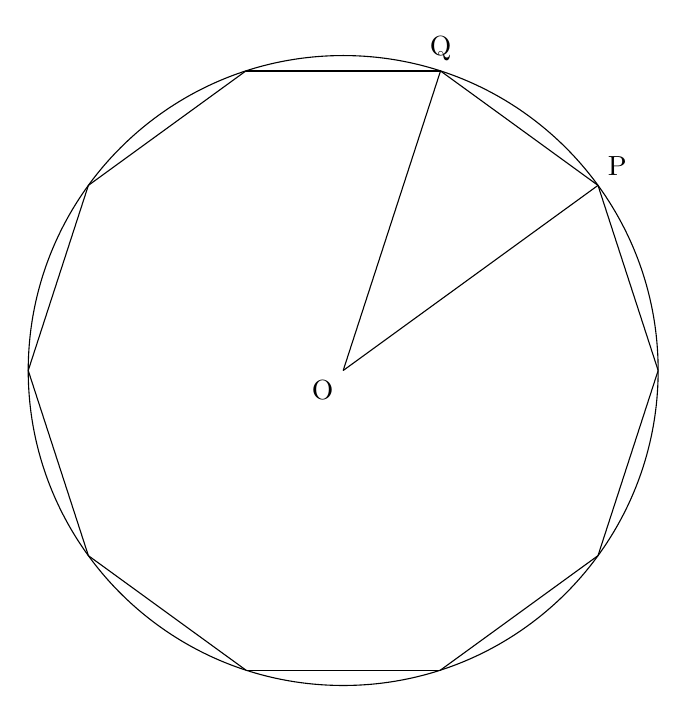
\begin{tikzpicture}[baseline={(A.base)}]
		\draw (0,0) circle [radius=4];
		\coordinate[label=below left:O] (O) at (0:0);
		\coordinate[label=above right:P] (P) at (36:4);
		\coordinate[label=above:Q] (Q) at (72:4);
		\coordinate (A) at (108:4);
		\coordinate (B) at (144:4);
		\coordinate (C) at (180:4);
		\coordinate (D) at (216:4);
		\coordinate (E) at (252:4);
		\coordinate (F) at (288:4);
		\coordinate (G) at (324:4);
		\coordinate (H) at (0:4);
		\draw (P) -- (Q);
		\draw (Q) -- (A);
		\draw (A) -- (B);
		\draw (B) -- (C);
		\draw (C) -- (D);
		\draw (D) -- (E);
		\draw (E) -- (F);
		\draw (F) -- (G);
		\draw (G) -- (H);
		\draw (H) -- (P);
		\draw (O) -- (P);
		\draw (O) -- (Q);
	\end{tikzpicture}
	\end{minipage}
	
	\item[(b)]
	\begin{align*}
		&\Limit[n]{\infty}{2nr\sin\frac{\pi}{n}} \\
		={}&\Limit[n]{\infty}{\frac{2nr\sin\frac{\pi}{n}}{\frac{\pi}{n}}\cdot\frac{\pi}{n}} \\
		={}&\limit[n]{\infty}\frac{\sin\frac{\pi}{n}}{\frac{\pi}{n}}\cdot\Limit[n]{\infty}{\frac{\pi}{n}\cdot2nr} \\
		\intertext{Let $m=\frac{\pi}{n}$. As $n\to\infty$, $m\to0$.}
		={}&\limit[m]{0}\frac{\sin m}{m}\cdot\limit{\infty}2\pi r \\
		={}&1\cdot2\pi r \\
		={}&\boxed{2\pi r}
	\end{align*}

	\item[(c)]
	Perimeter of a circle
\end{itemize}
\end{document}
